\documentclass{article}
\usepackage[utf8]{inputenc}
\usepackage{graphicx}
\usepackage{svg}
\usepackage{svg-extract}
\usepackage{geometry}
\usepackage{tabularx}
\usepackage{caption}
\usepackage{float}
\geometry{margin=1in} % Imposta i margini
\usepackage{titling} % Pacchetto aggiunto per gestire il titolo
\usepackage{ulem}
\usepackage{amsmath}
\usepackage{listings}
\usepackage{graphicx}

\title{Documentazione Sistema Di Gestione Del Ciclo Di Vita Di Una Pagina Wiki}
\author{Giuseppe Pollio, Mario Lombardo}
\date{Anno accademico 2023-2024}



\renewcommand{\maketitle}{%
	\begin{titlepage}
		\centering
		
\includegraphics[width=5cm]{logo_uni.png}\par\vspace{1cm}
		\huge\bfseries\thetitle\par
		\vspace{1cm}
		\Large\theauthor\par
		\vfill
		\large\thedate\par
	\end{titlepage}
}


\renewcommand{\contentsname}{Indice}

\begin{document}
	
	\maketitle
	
	\tableofcontents
	
	\newpage
	
	\section{Dominio del problema}
	\subsection{Introduzione}
	In questa soluzione, esaminiamo attentamente il problema per identificarne il dominio, con l'intento di sviluppare un diagramma che orienterà le nostre decisioni di progettazione a livello di codice.
	
		\subsection{Analisi dei requisiti}
		In questa sezione si analizza la traccia in maniera specifica con lo scopo di definire le funzionalità
		che la base di dati deve soddisfare. Individueremo le entità e le associazioni
		del mini-word, producendo la prima versione del modello concettuale che
		sarà poi rielaborato nelle fasi successive della progettazione.\\ \\
		{\itshape "Si sviluppi un sistema informativo, composto da una base di dati relazionale e da un applicativo Java dotato
			di GUI (Swing o JavaFX), per la gestione del ciclo di vita di una pagina di una wiki"}
		\vspace{0.5cm}
		\\
		{\itshape "Una pagina di una wiki ha un titolo e un testo. Ogni pagina è creata da un determinato autore. Il testo è
			composto di una sequenza di frasi. Il sistema mantiene traccia anche del giorno e ora nel quale la pagina è
			stata creata. Una frase può contenere anche un collegamento. Ogni collegamento è caratterizzato da una
			frase da cui scaturisce il collegamento e da un’altra pagina destinazione del collegamento."}
		\vspace{0.5cm}
		\\
		{\itshape "Il testo può essere modificato da un altro utente del sistema, che seleziona una o più delle frasi, scrive la sua	
			versione alternativa (modifica) e prova a proporla"}
		\vspace{0.5cm}
		
		
		Dall'introduzione individuiamo il mini-world da rappresentare, ovvero un \textit{"Sistema informativo per la gestione del ciclo di vita di una pagina di una wiki"}, e iniziamo a riconoscere la prima entità:
		\textbf{Page} avente come attributi \texttt{title} e \texttt{creation\_date}. 
		Inoltre una pagina della Wiki deve essere composta da un testo, a sua volta composto da una sequenza di frasi, e questo testo deve poter essere modificabile da un utente, individuiamo cos\`i un entità associata alla pagina: \textbf {PageText} contenente come attributi, la riga di testo \texttt{text} e un indice per l'ordinamento delle righe di testo \texttt{order\_num}. Invece di utilizzare un singolo attributo per salvare tutto il contenuto di una pagina l'utilizzo dell'entità \textbf{PageText} ottimizza molto le operazioni di modifica del testo poich\`e lavora su singole righe di testo invece di lavorare su l'intero contenuto.
		Una frase del testo di una pagina puo' contenere un collegamento ad un altra pagina, otteniamo questo comportamento aggiungendo all'entità \textbf{PageText} l'attributo \texttt{link} (attributo parziale) tenendo traccia del \texttt{page\_id} della Pagina alla quale ci riferiamo. Andiamo ad utilizzare il formato \texttt{\{page\_id:riga\_di\_testo\}} quando una riga di testo è un collegamento, sarà l'applicativo a mostrare solo la riga\_di\_testo e gestire il collegamento alla pagina.
		\\\\\\
		{\itshape "La modifica proposta verrà notificata all’autore del testo originale la prossima volta che utilizzerà il sistema.
			L’autore potrà vedere la sua versione originale e la modifica proposta. Egli potrà accettare la modifica (in
			quel caso la pagina originale diventerà ora quella con la modifica apportata), rifiutare la modifica (la pagina
			originale rimarrà invariata). La modifica proposta dall’autore verrà memorizzata nel sistema e diventerà
			subito parte della versione corrente del testo. Il sistema mantiene memoria delle modifiche proposte e anche
			delle decisioni dell’autore (accettazione o rifiuto)."}
		\vspace{0.5cm}
		\\
		{\itshape "Nel caso in cui si fossero accumulate più modifiche da rivedere, l’autore dovrà accettarle o rifiutarle tutte
			nell’ordine in ordine dalla più antica alla più recente"}
		\vspace{0.5cm}
		\\
		{\itshape "Gli utenti generici del sistema potranno cercare una pagina e il sistema mostrerà la versione corrente del
			testo e i collegamenti.
			Gli autori dovranno prima autenticarsi fornendo la propria login e password. Tutti gli autori potranno vedere
			tutta la storia di tutti i testi dei quali sono autori e di tutti quelli nei quali hanno proposto una modifica"}
		\vspace{0.5cm}
		
		
		Sarà necessario tenere traccia degli utenti della Wiki per poter permettere loro pubblicare nuove pagine e gestire le pagine esistenti (richiedendo modiche agli autori), da questo andiamo a creare l'entità \textbf{User}, alla quale sarà possibile accedere al sistema tramite una \textbf{password} e un \textbf{username}. Inoltre il sistema tiene conto del fatto che un utente possa essere un Gestore della Wiki tramite l'attributo \texttt{admin} (attributo parziale).
		All'entità \textbf{Page} individuiamo la necessità di possedere un autore inserendo l'attributo \textbf{author}. Le modifiche del testo di una pagina (\textbf {Page}) saranno salvate tramite le l'entità \textbf {PageUpdate} avente attributi: \textbf{status}, che indica lo stato della modifica, e un collegamento all'utente \textbf{User} autore della modifica (\texttt {author}). Le righe di testo da modificare sono individuate tramite l'entità \textbf {UpdatedText} che contiene l'attributo \texttt{text} che indica la "nuova riga di testo", un collegamento \texttt{link} (attributo parziale) e un collegamento all'entità \textbf{PageUpdate}.
		Quando una modifica viene inoltrata all'autore esso invece deve essere avvisato tramite una notifica, questa verrà gestita dall'entità \textbf{Notification} avente come attributi \texttt{status} (stato della notifica, \texttt{OPEN, CLOSED}), il tipo di notifica \texttt{type} (\texttt{REQUEST\_UPDATE, UPDATE\_ACCEPTED, UPDATE\_REJECTED}), \texttt{viewed} per indicare se la notifica è stata letta, e ovviamente, contiene le relazioni all'utente destinatario \textbf{User} e alla modifica del testo \textbf{PageUpdate}. 
		In fine \textit{Tutti gli autori potranno vedere tutta la storia di tutti i testi dei quali sono autori e di tutti quelli nei quali hanno proposto una modifica} sarà possibile per via delle relazioni \textbf{User} → \textbf{Page} usando l'attributo \texttt{author} contenuto in \textbf{Page}, e \textbf{PageUpdate} → \textbf{Page} usando l'attributo \texttt{page\_id} in \textbf{PageUpdate}.
		\\\\\\
		
		\newpage
		
		\subsection{Diagramma del Dominio del Problema}
		In seguito alle considerazioni espresse nella sezione precedente, si è prodotto il seguente class diagram del dominio del problema:
		\begin{center}
			\includegraphics[width=1\linewidth]{UML\_RISTRUTTURATO.drawio.png}
		\end{center}
		
		\subsection{Dizionari}
		{\subsubsection{Dizionario delle Entità}}
		
		\begin{table}[H]
			\centering
			\small % Riduci la dimensione del font
			\setlength{\tabcolsep}{6pt} % Riduci lo spazio tra le colonne
			\renewcommand{\arraystretch}{1.2} % Aumenta lo spazio tra le righe
			
			\begin{tabularx}{\textwidth}{|l|X|X|}
				\hline
				\textbf{Entità} & \textbf{Descrizione} & \textbf{Attributi} \\
				\hline
				User & Account Utente della wiki. & 
				\textbf{Username}(Stringa): nome identificativo dell'account utente.
				
				\textbf{Password}(Stringa): password necessaria
				per accedere all’account utente. \\
				\hline
				Page & Pagina presente sulla wiki. & 
				\textbf{Title}(Stringa): Titolo della pagina.
				
				\textbf{CreationDate}(Data/Timestamp): Data e ora di creazione della pagina.
				\\
				\hline
				PageText & Frase di una Pagina (\textbf{Page}). &
				\textbf{Text}(Stringa): Contenuto della frase.
				
				\textbf{Order\_num}(Intero): Ordinamento della frase all'interno del testo complessivo.
				\\
				\hline
				PageUpdate & Modifica proposta ad pagina da parte di un altro utente. & 
				\textbf{Status}(Intero): Stato della richiesta di modifica.
				\\
				\hline
				UpdatedText & Nuovo testo proposto durante la modifica (\textbf{PageUpdate}). & 
				\textbf{Text}(Stringa): Contenuto della riga di testo.
				
				\textbf{Order\_num}(Intero): Ordinamento della frase all'interno del testo complessivo.
				\\
				\hline
				Notification & Notifiche di un \textbf{Utente (User)}.& 
				\textbf{Status}(Intero): Stato della notifica. (\texttt{OPEN, CLOSED})
				
				\textbf{Viewed}(Booleano): Stato di lettura di una notifica.
				
				\textbf{Type}(Intero): Tipologia di notifica. (\texttt{REQUEST\_UPDATE, UPDATE\_ACCEPTED, UPDATE\_REJECTED})
				\\
				\hline
				Admin & Specializzazione parziale di un utente, un amministratore pu\`o modificare ed eliminare le pagine di altri utenti senza dover prima inviare una notifica di accettazione delle modifiche.& 
				\\
				\hline
				Link & Specializzazione parziale di una riga di testo che rappresent\`a se una riga di testo \`e un collegamento o meno.& 
				\\
				\hline
				
			\end{tabularx}
			
		\end{table}
		
		{\subsubsection{Dizionario delle Associazioni}}
		
		\begin{table}[H]
			\centering
			\small % Riduci la dimensione del font
			\setlength{\tabcolsep}{6pt} % Riduci lo spazio tra le colonne
			\renewcommand{\arraystretch}{1.2} % Aumenta lo spazio tra le righe
			
			
			\begin{tabularx}{\textwidth}{|l|l|X|}
				\hline
				\textbf{Associazione} &\textbf{Tipologia}  & \textbf{Descrizione} \\
				\hline
				Autore Pagina & uno-a-molti  & Associa ad ogni pagina (Page) un utente (User) che ne rappresenta l'autore
				\\
				\hline
				Autore Modifica & uno-a-molti  & Associa ad ogni modifica (PageUpdate) un utente (User) che ne rappresenta l'autore
				\\
				\hline
				Testo Pagina & uno-a-molti  & Associa ad ogni pagina (Page) tutto il testo (PageText) appartenente a quella determinata pagina.
				\\
				\hline
				Testo Modifica & uno-a-molti  & Associa ad ogni modifica (PageUpdate) tutto il testo (UpdatedText) appartenente a quella determinata modifica.
				\\
				\hline
				Proprietario Notifica & uno-a-molti  & Associa ad ogni notifica (Notification) un utente (User) che ne rappresenta l'autore.
				\\
				\hline
				PageUpdate Notifica & uno-a-molti  & Associa ad ogni notifica (Notification) una modifica (PageUpdate) che ne aiuta a rappresentare il contenuto.
				\\
				\hline
				Page PageUpdate & uno-a-molti  & Associa ad ogni Modifica proposta (PageUpdate), La pagina (Page) per cui \`e stata proposta. 
				\\
				\hline
			\end{tabularx}
			
			
			
		\end{table}
		
		\newpage
		
		\section{Impementazione e Dominio della Soluzione}
		
		In questa sezione, illustreremo l'architettura dell'applicazione e i vari pattern utilizzati, fornendo occasionali annotazioni implementative. Abbiamo scelto di escludere la trattazione del codice effettivo, il quale è disponibile nella documentazione JavaDoc del codice sorgente e, naturalmente, nel sorgente stesso.
		
		\subsection{Architettura BCED}
		
		L'applicazione è stata progettata seguendo i principi dell'architettura {\itshape {Boundary-Control-Entity con estensione Database}}, nota come BCED. Il pattern BCED fornisce una struttura ben organizzata per separare le diverse responsabilità all'interno di un software, basandosi su quattro componenti principali
		
		
		\subsubsection{Boundary}
		Il componente boundary corrisponde all'interfaccia dell'applicazione che si occupa di far comunicare applicazione e utente attravero il controller. All'interno del codice della wiki questo componente \`e implementato attraverso il package \textbf{GUI}.

		\subsubsection{Control} Questo componente implementato attraverso il package \textbf{Controllers} gestisce un ruolo di controllo  e coordinazione sull'intera applicazione. Né la Boundary né l'Entity sono autorizzate a comunicare se non tramite il controller.
		
		\subsubsection{Entity}
		Per Entity si intende l'insieme delle informazioni da memorizzare durante l'esecuzione che sono di interesse nel dominio. Nel contesto di un'applicazione, essa è rappresentata dal modello di dati interno. \\\\
		Questo componente \`e stato definito attravero il pagacke \textbf{Model}.
		
		\subsubsection{Database}
		Nel contesto della nostra applicazione usiamo come database Postgres. Il database funge da posto in cui conservare i dati nel lungo termine, la connessione tramite dabtabase \`e stata implementata tramite due package: \textbf{wiki.DAOImplementations} e \textbf{database}
		
		
	\subsection {Controller}
	Il controller come gi\`a detto precedentemente \`e si occupa di gestire tutta la logica dell'applicazione, nell'applicazione questa componente \`e stata integrata tramite il package \textbf{Controllers} a sua volta contente una singola classe: \textbf{WikiController.java}. Nello specifico nella nostra applicazione le funzioni principali dell'WikiController sono:
	
	\begin{itemize}
		\item \textbf{Gestione e Controllo del model}: Nel controller sono contenuto tutte le istanze di classi del model durante l'esecuzione.
		
		\item \textbf{Comunicazione r/w col Database}: Il controller si occupa di comunicare col database e di inserire o prendere dati da esso per poi salvarli in locale, in maniera temporanea.
		
		\item \textbf{Comunicazione della GUI}: La GUI tramite callback invia informazioni al controller, in modo da poter poi eseguire azioni sul database e/o model.
		\\\\
		La GUI vicevera riceve informazioni dal controller rispetto a cosa deve mostrare all'utente
	\end{itemize}
	
	
	\subsection{Model}
	Tutte le entit\`a che sono state identificate nel dominio nella sezione \textbf{Dominio del problema} sono state tradotte in classi all'interno del package \textbf{Models} tuttavia non sono state tradotte esplicitamente le relazioni fra di esse. L'organizzazione del model piuttosto che essere come visto spesso un "carica tutto" si \`e deciso di utilizzare la tecnica del lazy loading, ossia piuttosto che prendere tutti i dati dal database assieme, si andranno a prendere solo i dati che saranno necessari in quel momento, questa tecnica molto utilizzata nei programmi pi\`u moderni permette di limitare l'utilizzo di memoria e i tempi di caricamento.
	\\
	Dato l'utilizzo del lazy loading l'unica istanza presente all'interno del controller \`e:
	
	\begin{itemize}
		\item \textbf{User loggedUser}: Istanza di \textbf{User} che rappresenta l'utente attualmente loggato. All'interno dell'istanza sono presenti anche le notifiche.
	\end{itemize}
	
	Il resto dei dati verr\`a caricato in modo dinamico, ad esempio se apro una determinata pagina della wiki saranno presi dal database in tempo reale solo i dati che servono al funzionamento di quella pagina, tuttavia una volta cambiata pagina i dati precedenti verranno cancellati dalla memoria.


	\subsection{Database e DAO}
	Per implementare la comunicazione tra l'applicazione e il database, è stato scelto il pattern DAO (\textit{Data Access Object}). Questo pattern propone la creazione di un'interfaccia astratta di comunicazione tra l'applicativo e il database. Il software è quindi progettato per interagire esclusivamente attraverso questa interfaccia, evitando qualsiasi dipendenza da un'applicazione specifica. Ciò consente all'applicativo di essere indipendente, senza avere conoscenza specifica sul database con cui sta interagendo.
	\\\\
	Il package DAO contiene l'interfaccia menzionata, rappresentata da una serie di interfacce Java, una per ogni entità del modello (e quindi del dominio del problema). Ciascuna interfaccia DAO definisce la firma delle operazioni eseguibili per l'entità corrispondente.
	\\\\
	La connessione al database viene effettuata tramite il package \textbf{database}, il database scelto \`e PostgreSQL.
	
	\subsection{Interfaccia Utente}
	L'interfaccia utente \`e stata quasi del tutto progettata a mano visto che molti compontenti di essa vengono generati dinamicamente durante l'utilizzo dell'applicazione. Per la GUI \`e stata utilizata la libreria Java Swing con l'implementazione di \textbf{Flatlaf} una libreria che ne migliora l'aspetto.

	\newpage

	\subsection{Diagramma della Soluzione}
	\begin{figure}[htbp]
		\centering
		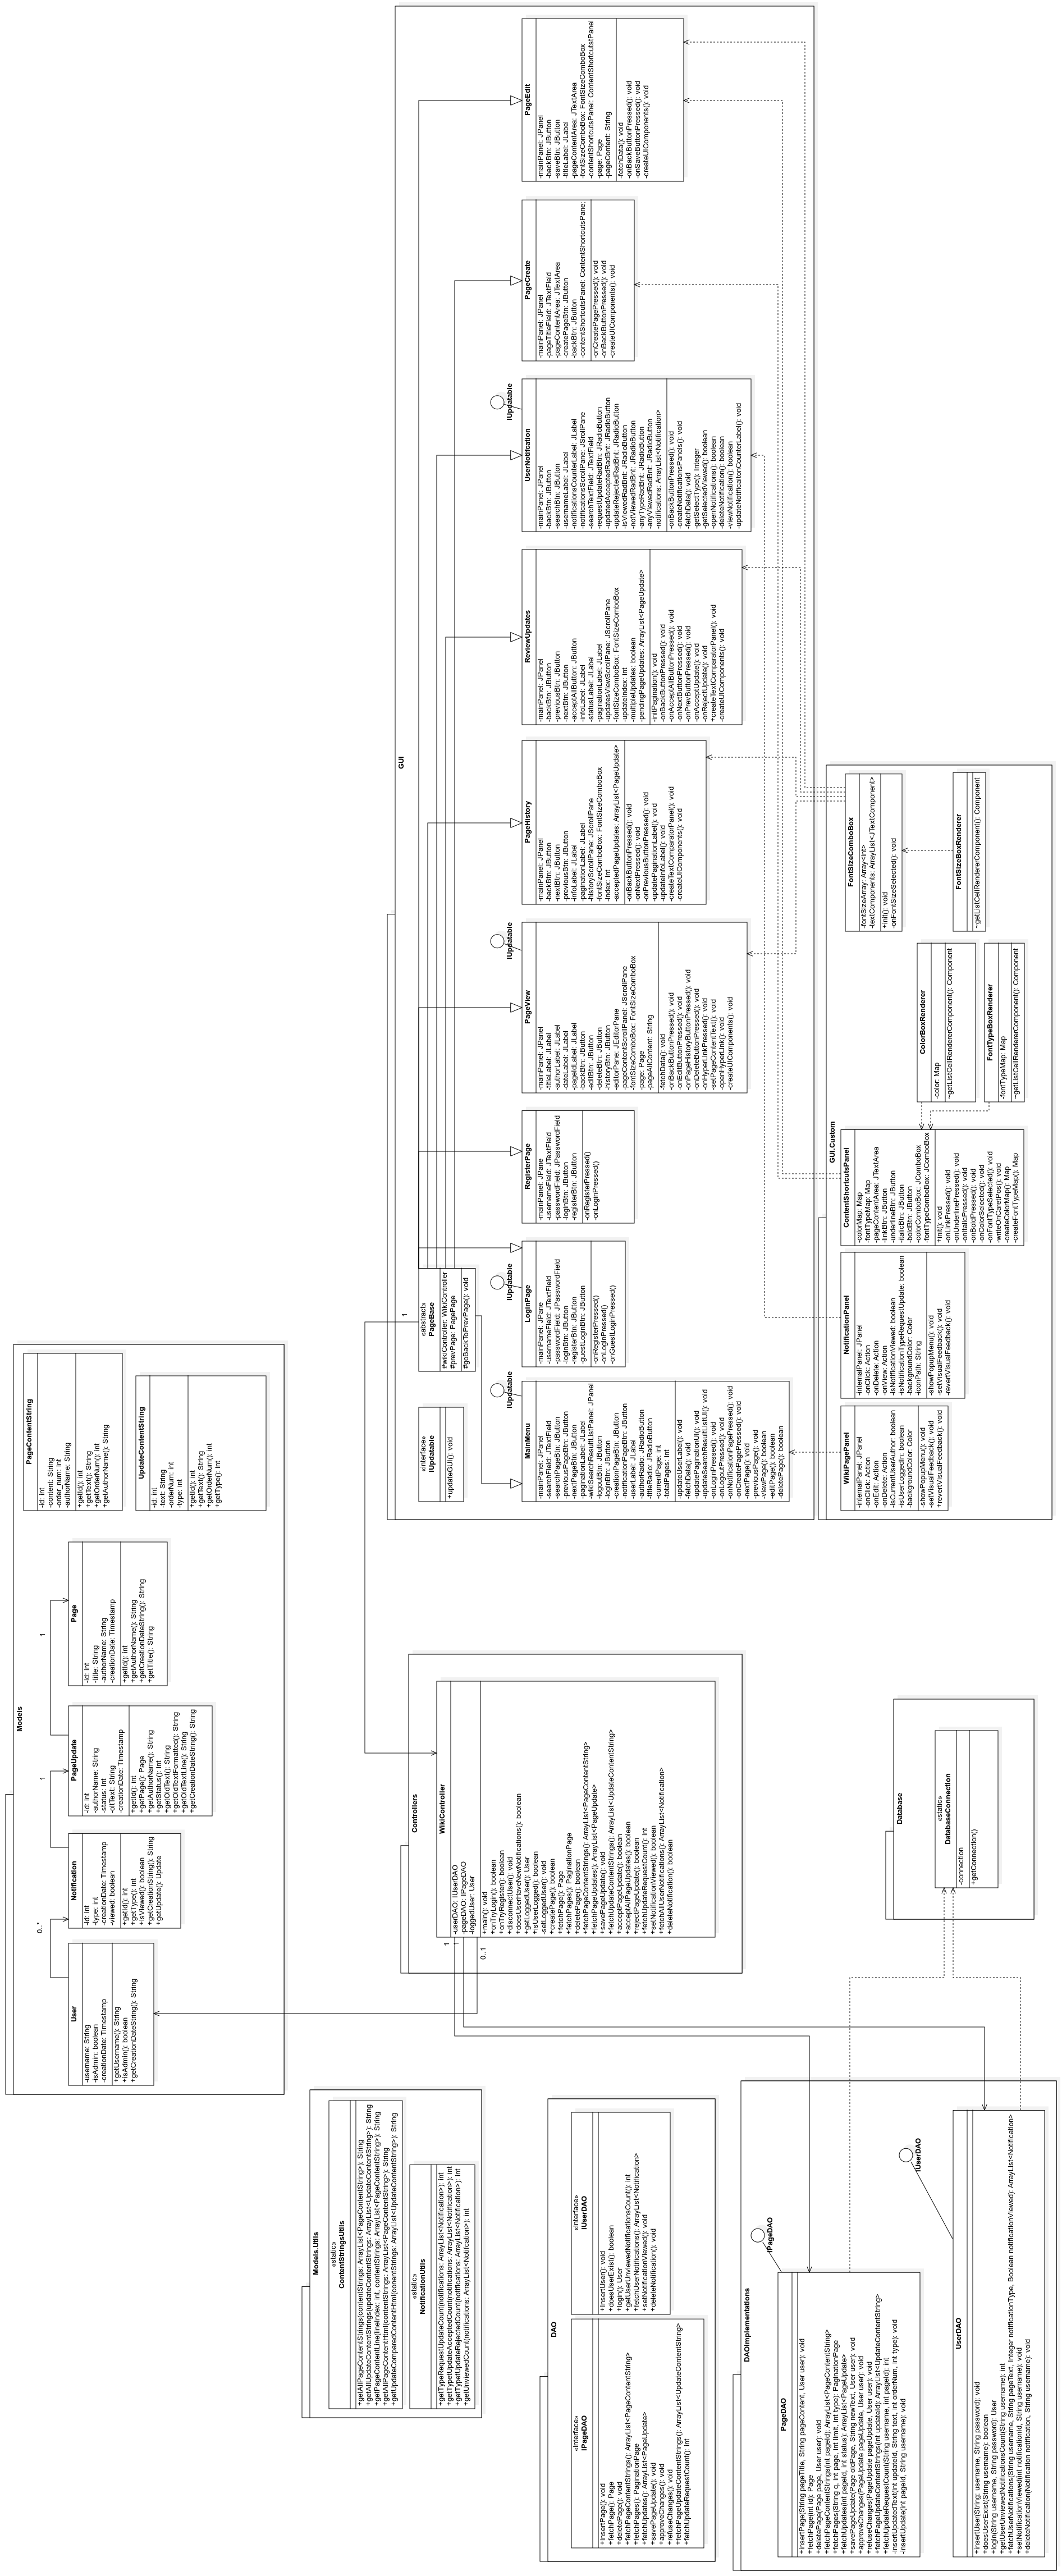
\includegraphics[width=0.7\textwidth,height=0.7\textheight,keepaspectratio]{solution_diagram.png}
		\label{fig:10}
	\end{figure}


	\newpage

	
	\section{Overview dell'Applicazione}
	Avendo parlato del funzionamento esterno dell'applicazione ora verr\`a presentato un "tour" guidato all'interno di essa, pagina per pagina. Specificandone tutte le funzionalit\`a.
	
	\subsubsection{LoginPage}
	
	\begin{figure}[htbp]
		\centering
		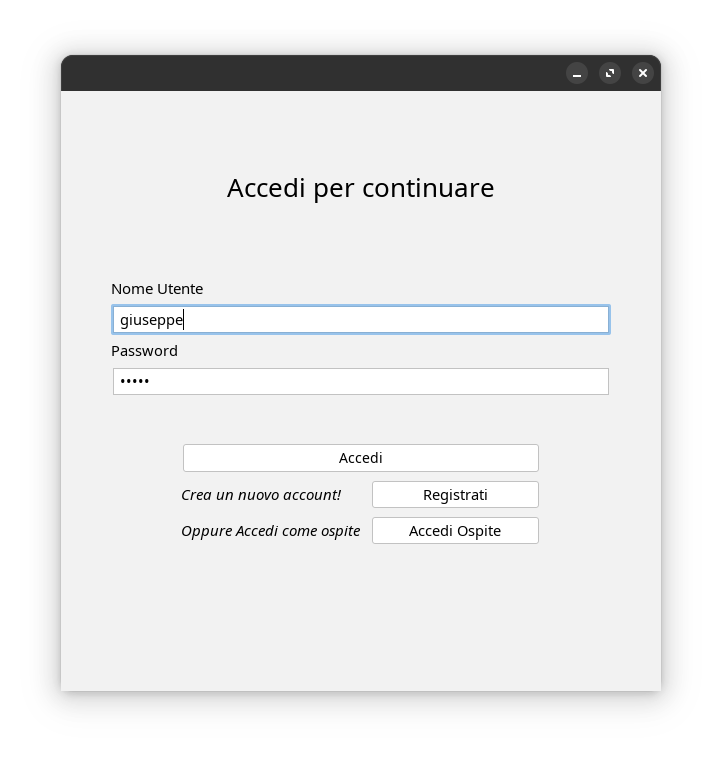
\includegraphics[width=0.8\textwidth,height=0.8\textheight,keepaspectratio]{login_page.png}
		\caption{L'utente in questo caso ha gi\`a inserito i propri dati.}
		\label{fig:1}
	\end{figure}
	
	L'applicazione ha come sua view iniziale la \textbf{LoginPage}. Qui l'utente pu\`o decidere se continuare col proprio account, inserendo i propri dati, registrarsi aprendo la view \textbf{RegisterPage} o accedere alla wiki come ospite.
	\\\\
	Il primo utente ad iscriversi riceve un account {\itshape{Admin}}. In grado di modificare ed eliminare pagine senza richiedere il permesso dell'autore.
	
	\newpage
	
	\subsubsection{RegisterPage}
	
	\begin{figure}[htbp]
		\centering
		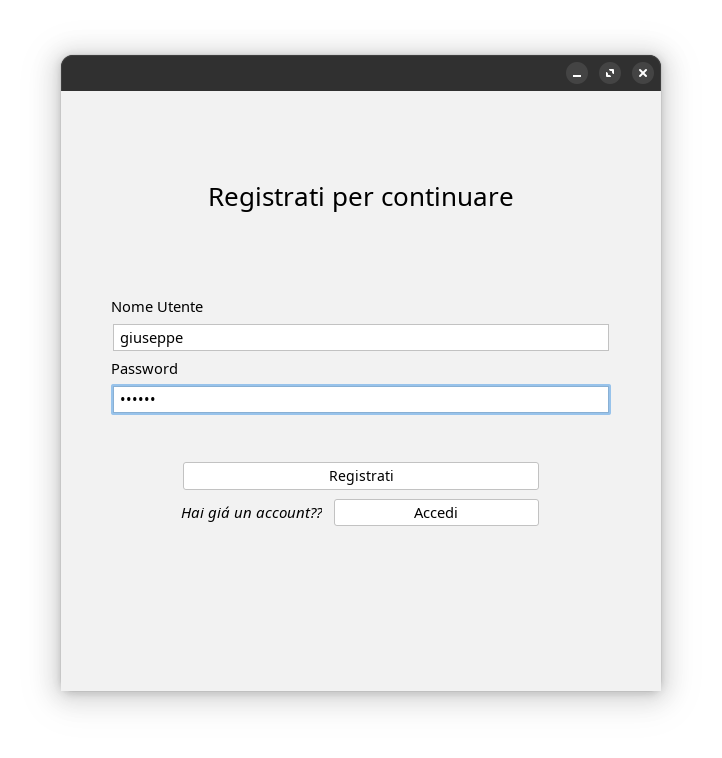
\includegraphics[width=0.8\textwidth,height=0.8\textheight,keepaspectratio]{register_page.png}
		\caption{RegisterPage}
		\label{fig:2}
	\end{figure}
	
	In questa pagine \`e possibile registrarsi alla wiki inserendo un proprio nome utente e password.
	
	\textbf{Nota}: Sia la password che il nome utente hanno dei caratteri minimi, inoltre il nome utente \`e unico per ogni utende della wiki e non \`e modificabile.
	
	\newpage
	
	\begin{figure}[htbp]
		\centering
		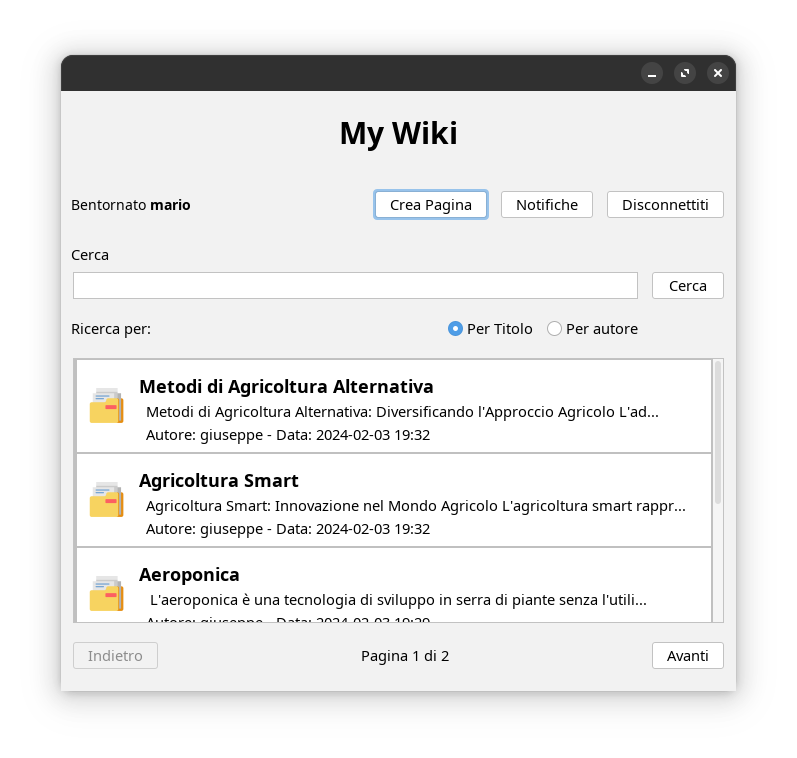
\includegraphics[width=0.8\textwidth,height=0.8\textheight,keepaspectratio]{ main_menu.png}
		\caption{MainMenu}
		\label{fig:3}
	\end{figure}
	
	Questa \`e la pagina centra dalla wiki e anche un p\`o il suo centro di controllo da qui sono possibili fare le seguenti azioni:
	
	\begin{itemize}
		\item Visualizzare tutte le pagine presenti sulla wiki.
		
		\item Creare nuove pagine \textbf{se loggato} attravero la pagina \textbf{PageCreate}.
		
		\item Leggere le proprie notifiche \textbf{se loggato} attraverso la pagina \textbf{UserNotifications}.
	\end{itemize}
	
	\newpage
	
	{\subsubsection{PageView}}
	
	\begin{figure}[htbp]
		\centering
		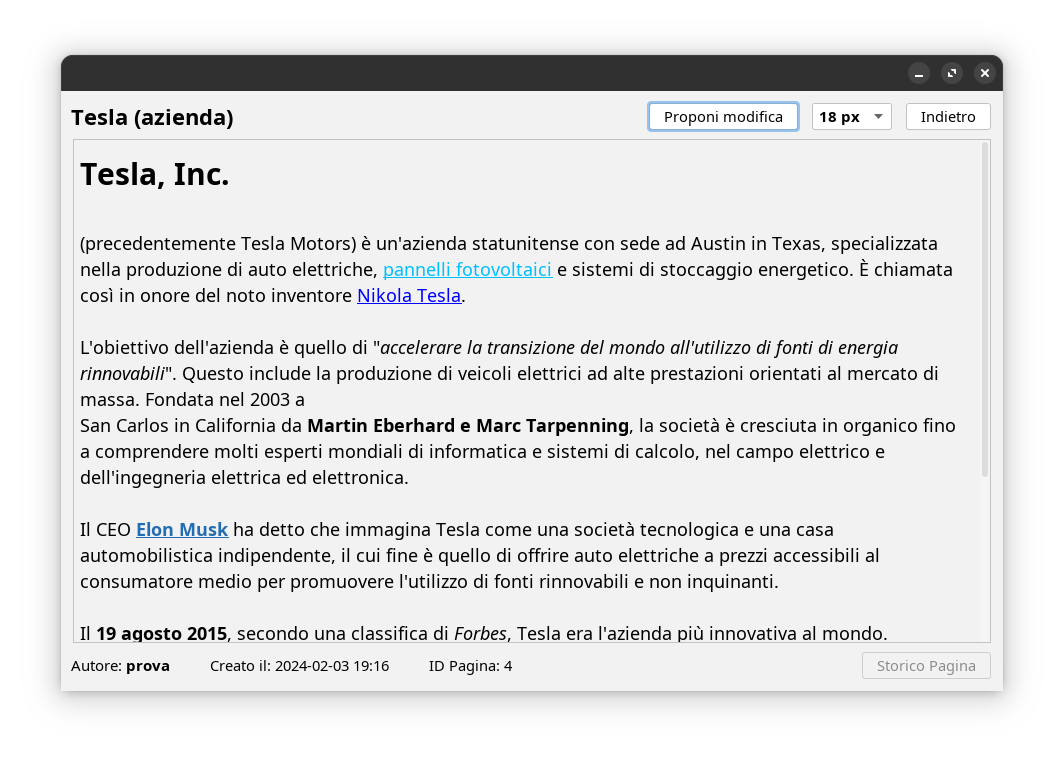
\includegraphics[width=0.8\textwidth,height=0.8\textheight,keepaspectratio]{page_view.png}
		\caption{In figura \`e mostrata una pagina con la maggior parte delle funzioni presenti nell'editor della wiki}
		\label{fig:4}
	\end{figure}
	
	In questa finestra \`e possibile visualizzare una pagina presente sulla wiki.\\
	L'applicazione gestisce il testo utilizzando il linguaggio di markup {\textbf{HTML (HyperText Markup Language)}}. \\\\
	
	L'utente ha accesso alle seguenti azioni:
	
	\begin{itemize}
		\item Proporre una modifica alla pagina attraverso a la pagina \textbf{PageEdit}.
		
		\item Modificare la grandezza del font.
		
		\item Visualizzare lo storico delle modifiche della pagina andando alla pagina \textbf{PageHistory}.
	\end{itemize}
	
	
	\newpage
	
	{\subsubsection{PageCreate}}
	
		\begin{figure}[htbp]
		\centering
		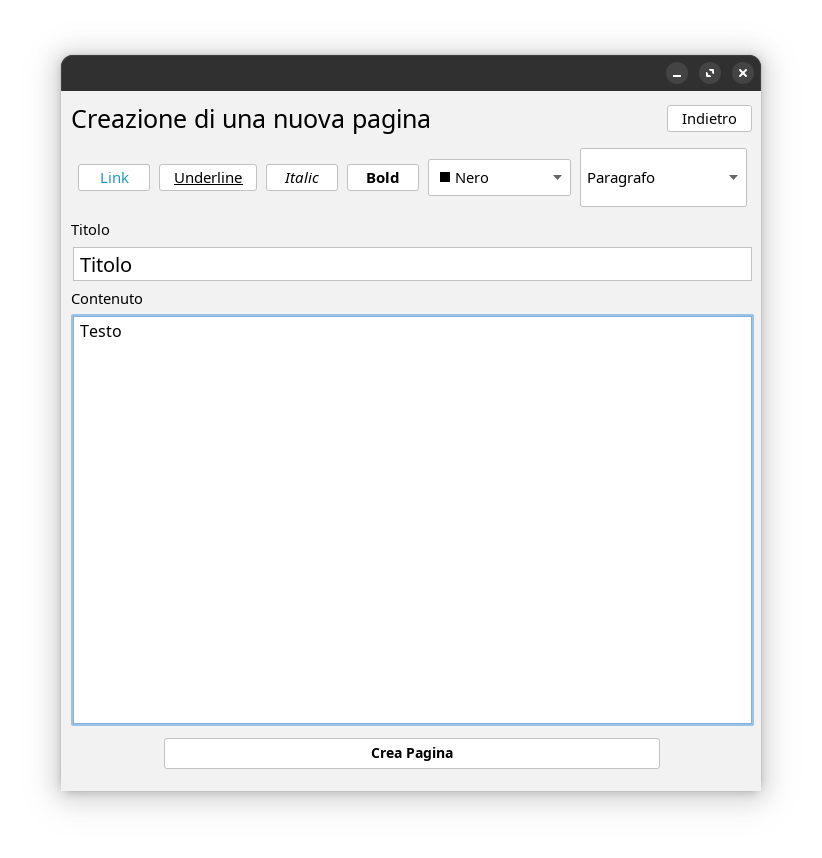
\includegraphics[width=0.8\textwidth,height=0.8\textheight,keepaspectratio]{page_create.png}
		\caption{Finestra in cui \`e possibile creare una nuova pagina}
		\label{fig:5}
	\end{figure}
	
	\newpage
	
	
	\subsubsection{PageEdit}
	\begin{figure}[htbp]
		\centering
		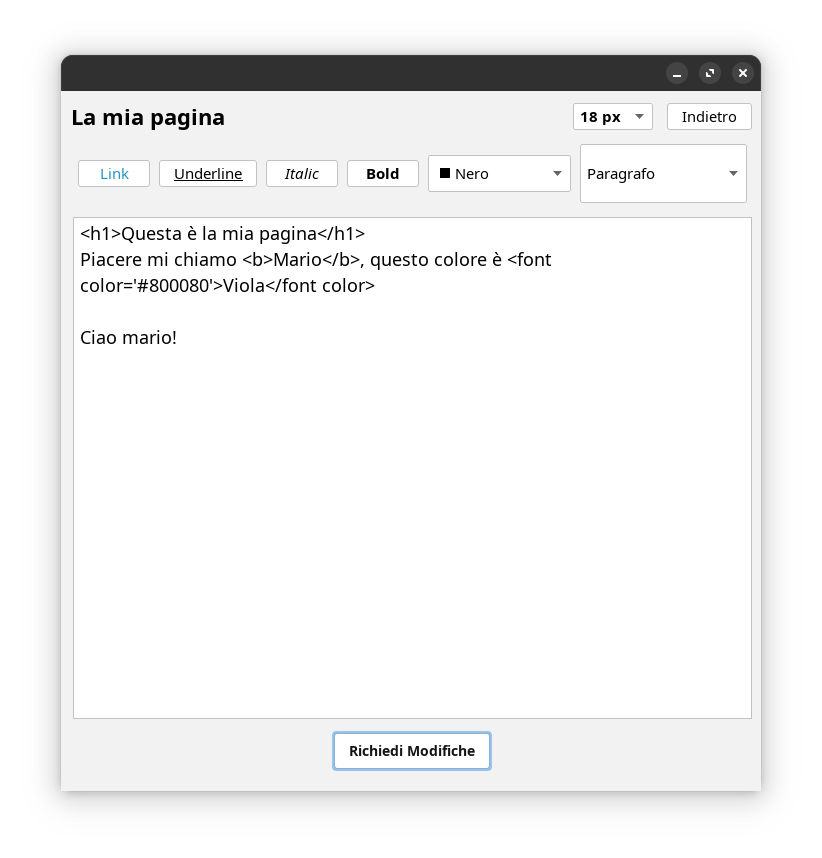
\includegraphics[width=0.8\textwidth,height=0.8\textheight,keepaspectratio]{page_edit.png}
		\caption{PageEdit}
		\label{fig:6}
	\end{figure}
	
	In questa pagina \'e possibile modificare una pagina a proprio piacimento.
	\\\\
	\textbf{Nota}: Questa azione non modificher\`a mai la pagina direttamente ma creer\`a sempre prima una richiesta all'utente proprietario della pagina. Tuttavia se l'utente che richiede una modifica \`e un {\itshape{Admin}} o il proprietario della pagina, la modifica verra accettata automaticamente.
	
	
	\newpage
	
	{\subsubsection{PageHistory}}
	\begin{figure}[htbp]
		\centering
		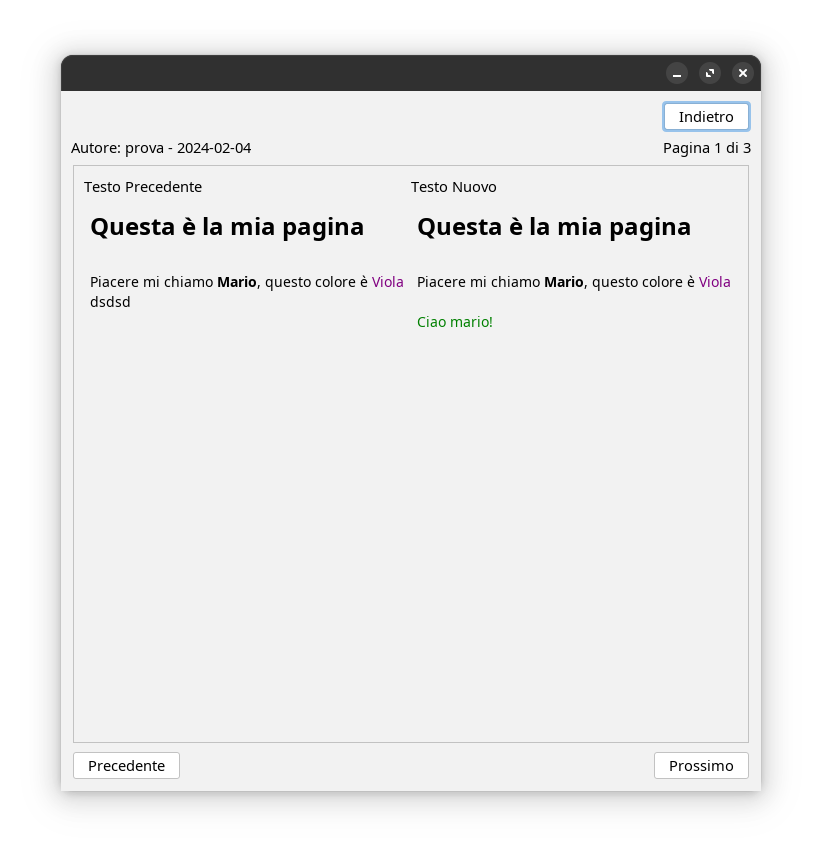
\includegraphics[width=0.8\textwidth,height=0.8\textheight,keepaspectratio]{page_history.png}
		\caption{Figura che mostra la cronologia delle modifiche di una pagina}
		\label{fig:7}
	\end{figure}
	
	\newpage
	
	{\subsubsection{UserNotifications}}
		\begin{figure}[htbp]
		\centering
		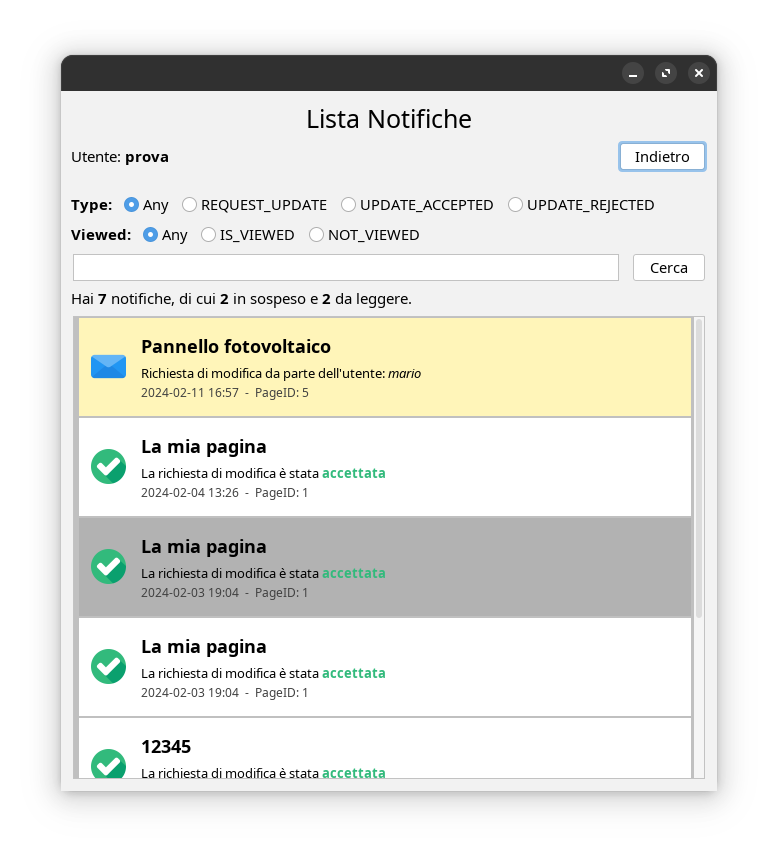
\includegraphics[width=0.8\textwidth,height=0.8\textheight,keepaspectratio]{user_notifications.png}
		\caption{In giallo, modifiche non lette.}
		\label{fig:8}
	\end{figure}
	
	In questa pagina sono mostrate tutte le notifiche di un utente, tra cui anche le richieste di modifica pagina che quando cliccate portano alla pagina \textbf{ReviewUpdates}.
	
	\newpage
	
	\subsubsection{ReviewUpdates}
	\begin{figure}[htbp]
		\centering
		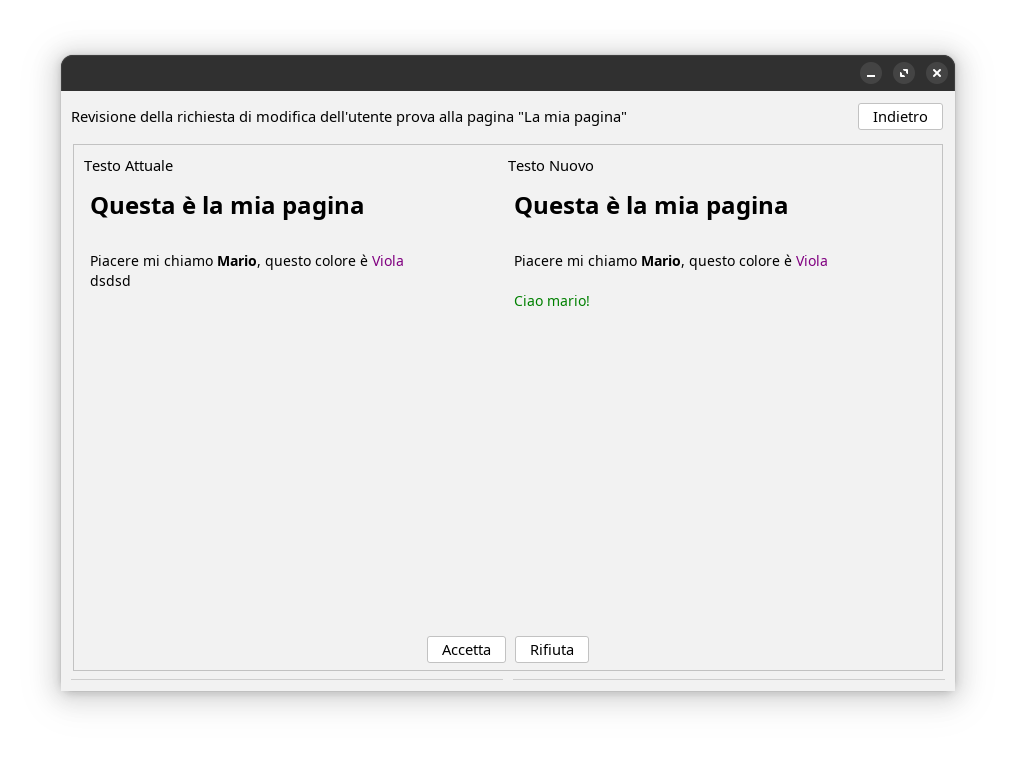
\includegraphics[width=0.8\textwidth,height=0.8\textheight,keepaspectratio]{review_updates.png}
		\caption{ReviewUpdates}
		\label{fig:9}
	\end{figure}
	
	Pagina in cui accettare o modificare le modifiche proposte ad una tua pagina. Le modifiche possono anche essere accettate in bulk (e pi\`u di una).	
	
	\newpage
	
	\section{Sequence Diagram}
	
	\subsection{Login (senza notifiche)}
		\begin{figure}[htbp]
		\centering
		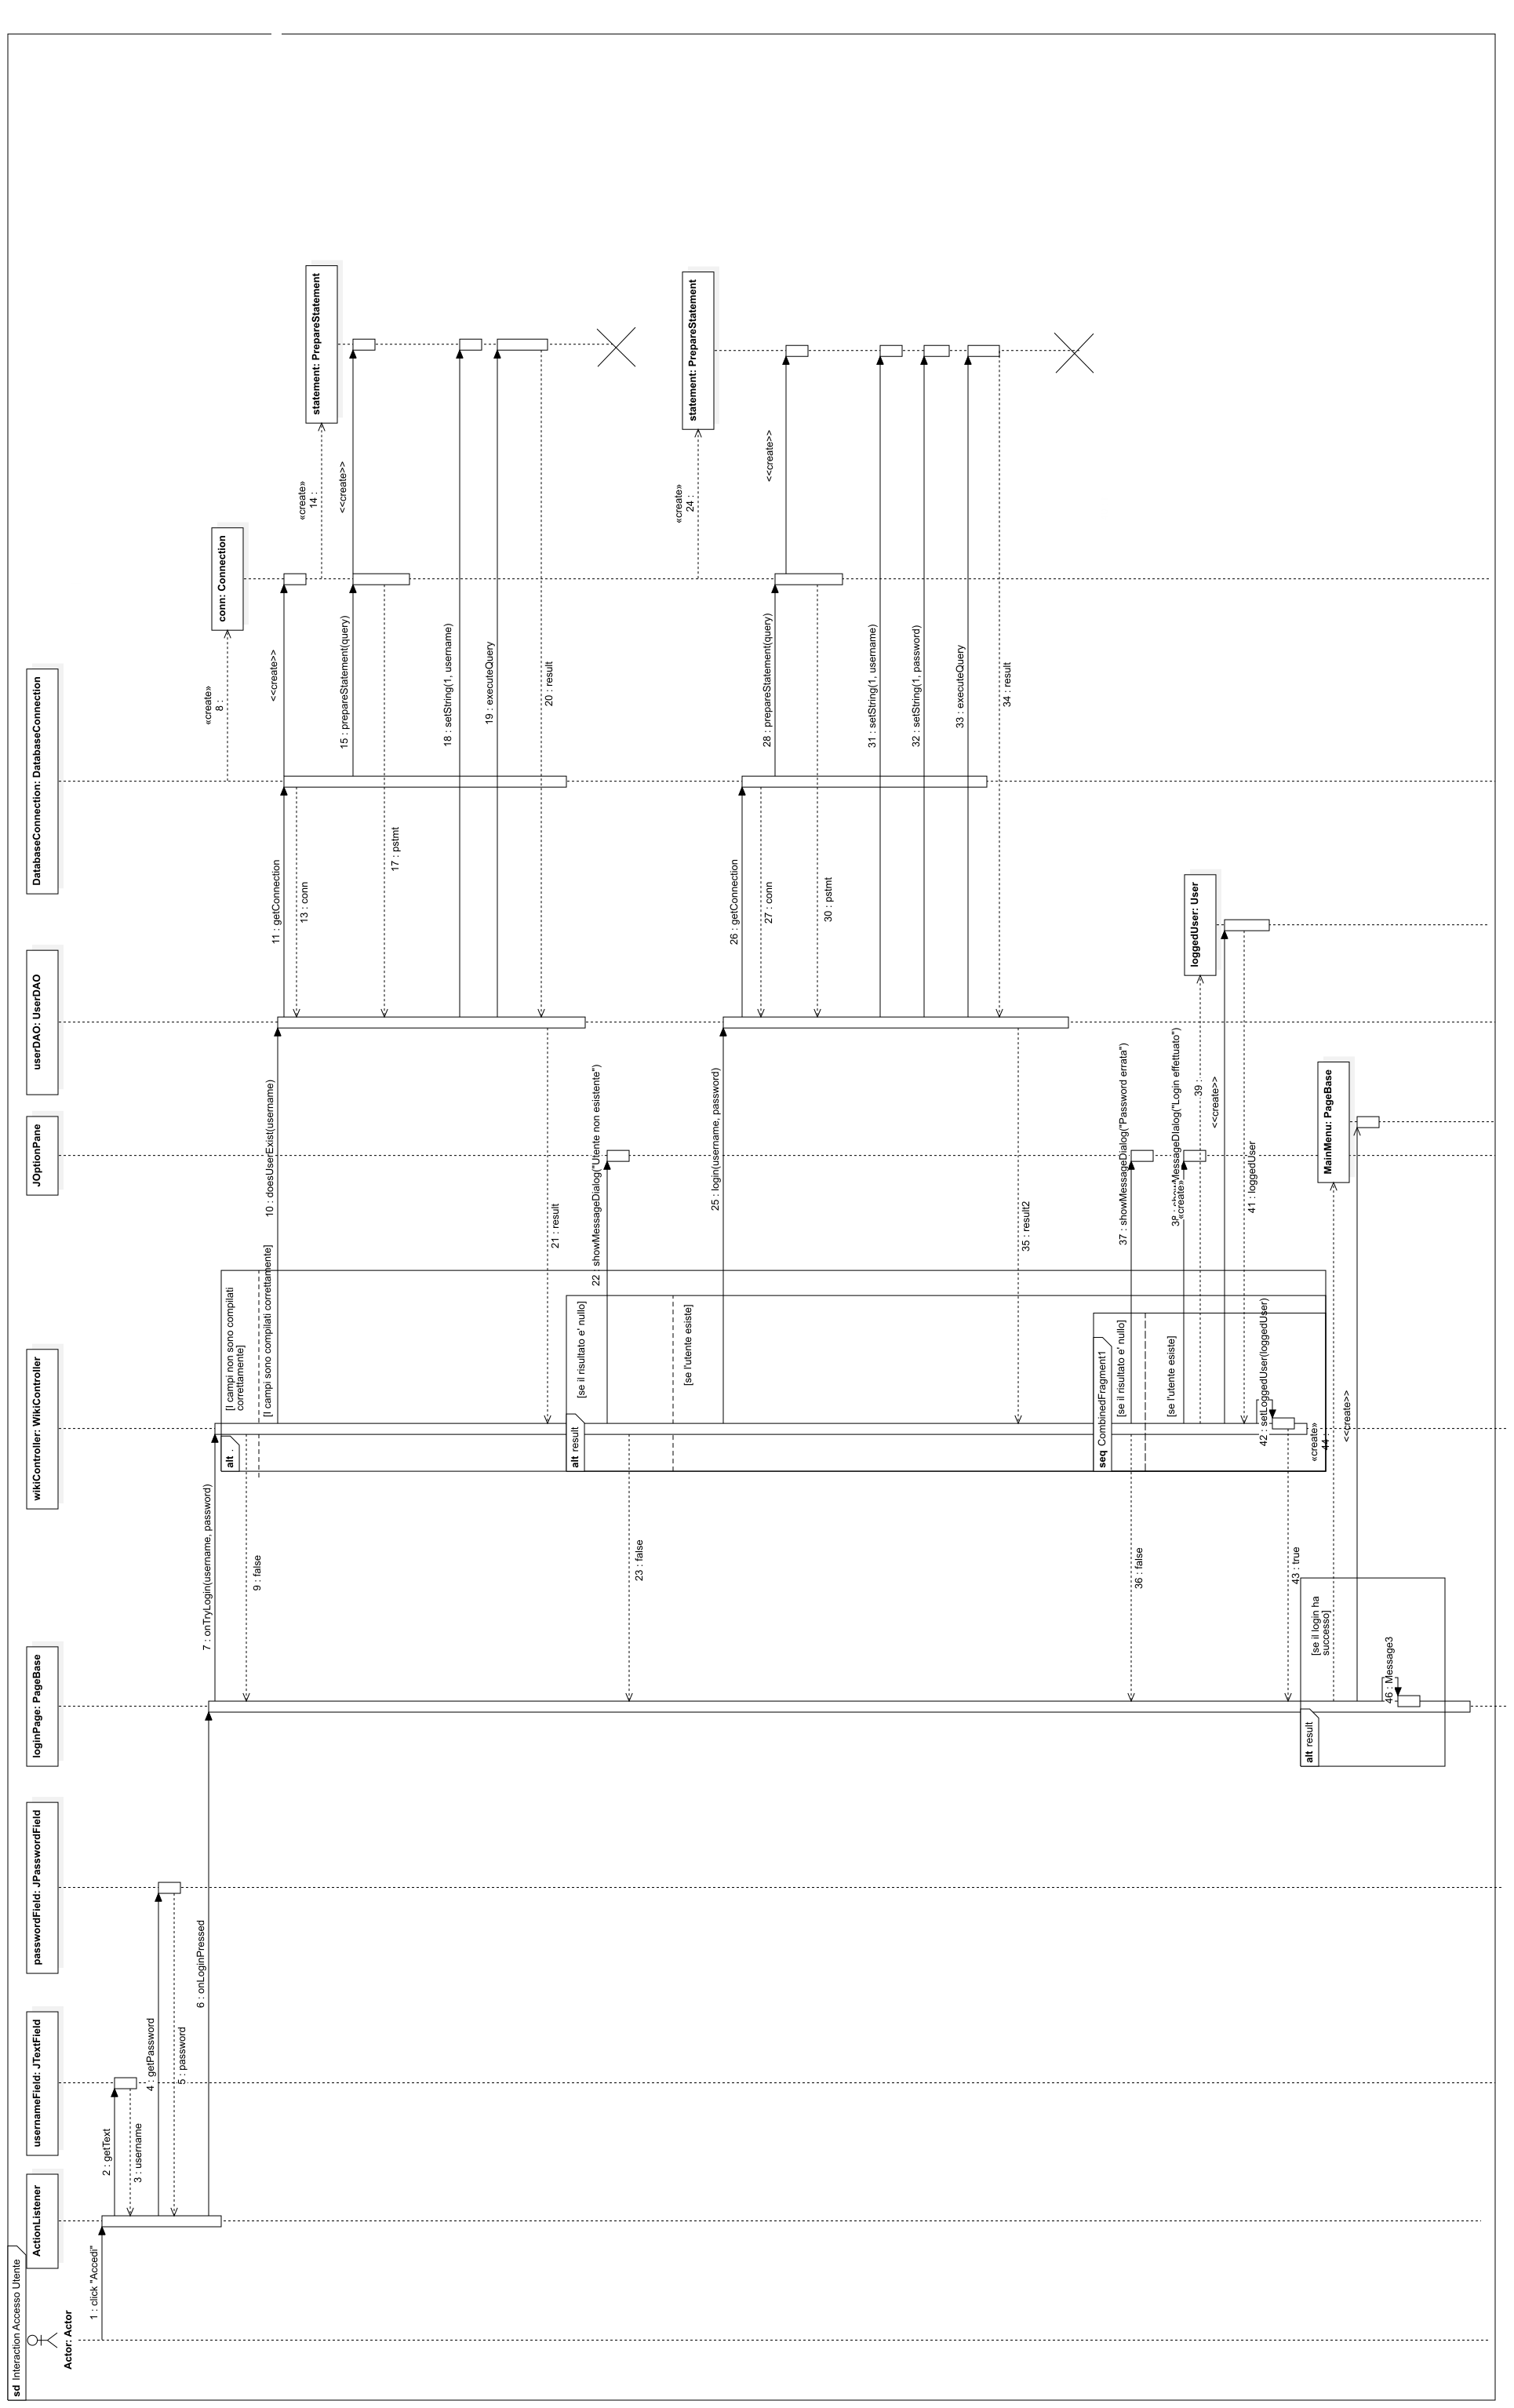
\includegraphics[width=0.7\textwidth,height=0.7\textheight,keepaspectratio]{sequence_login.png}
		\label{fig:10}
	\end{figure}
	
	\newpage
	
	\subsection{Modifica Pagina}
	\begin{figure}[htbp]
		\centering
		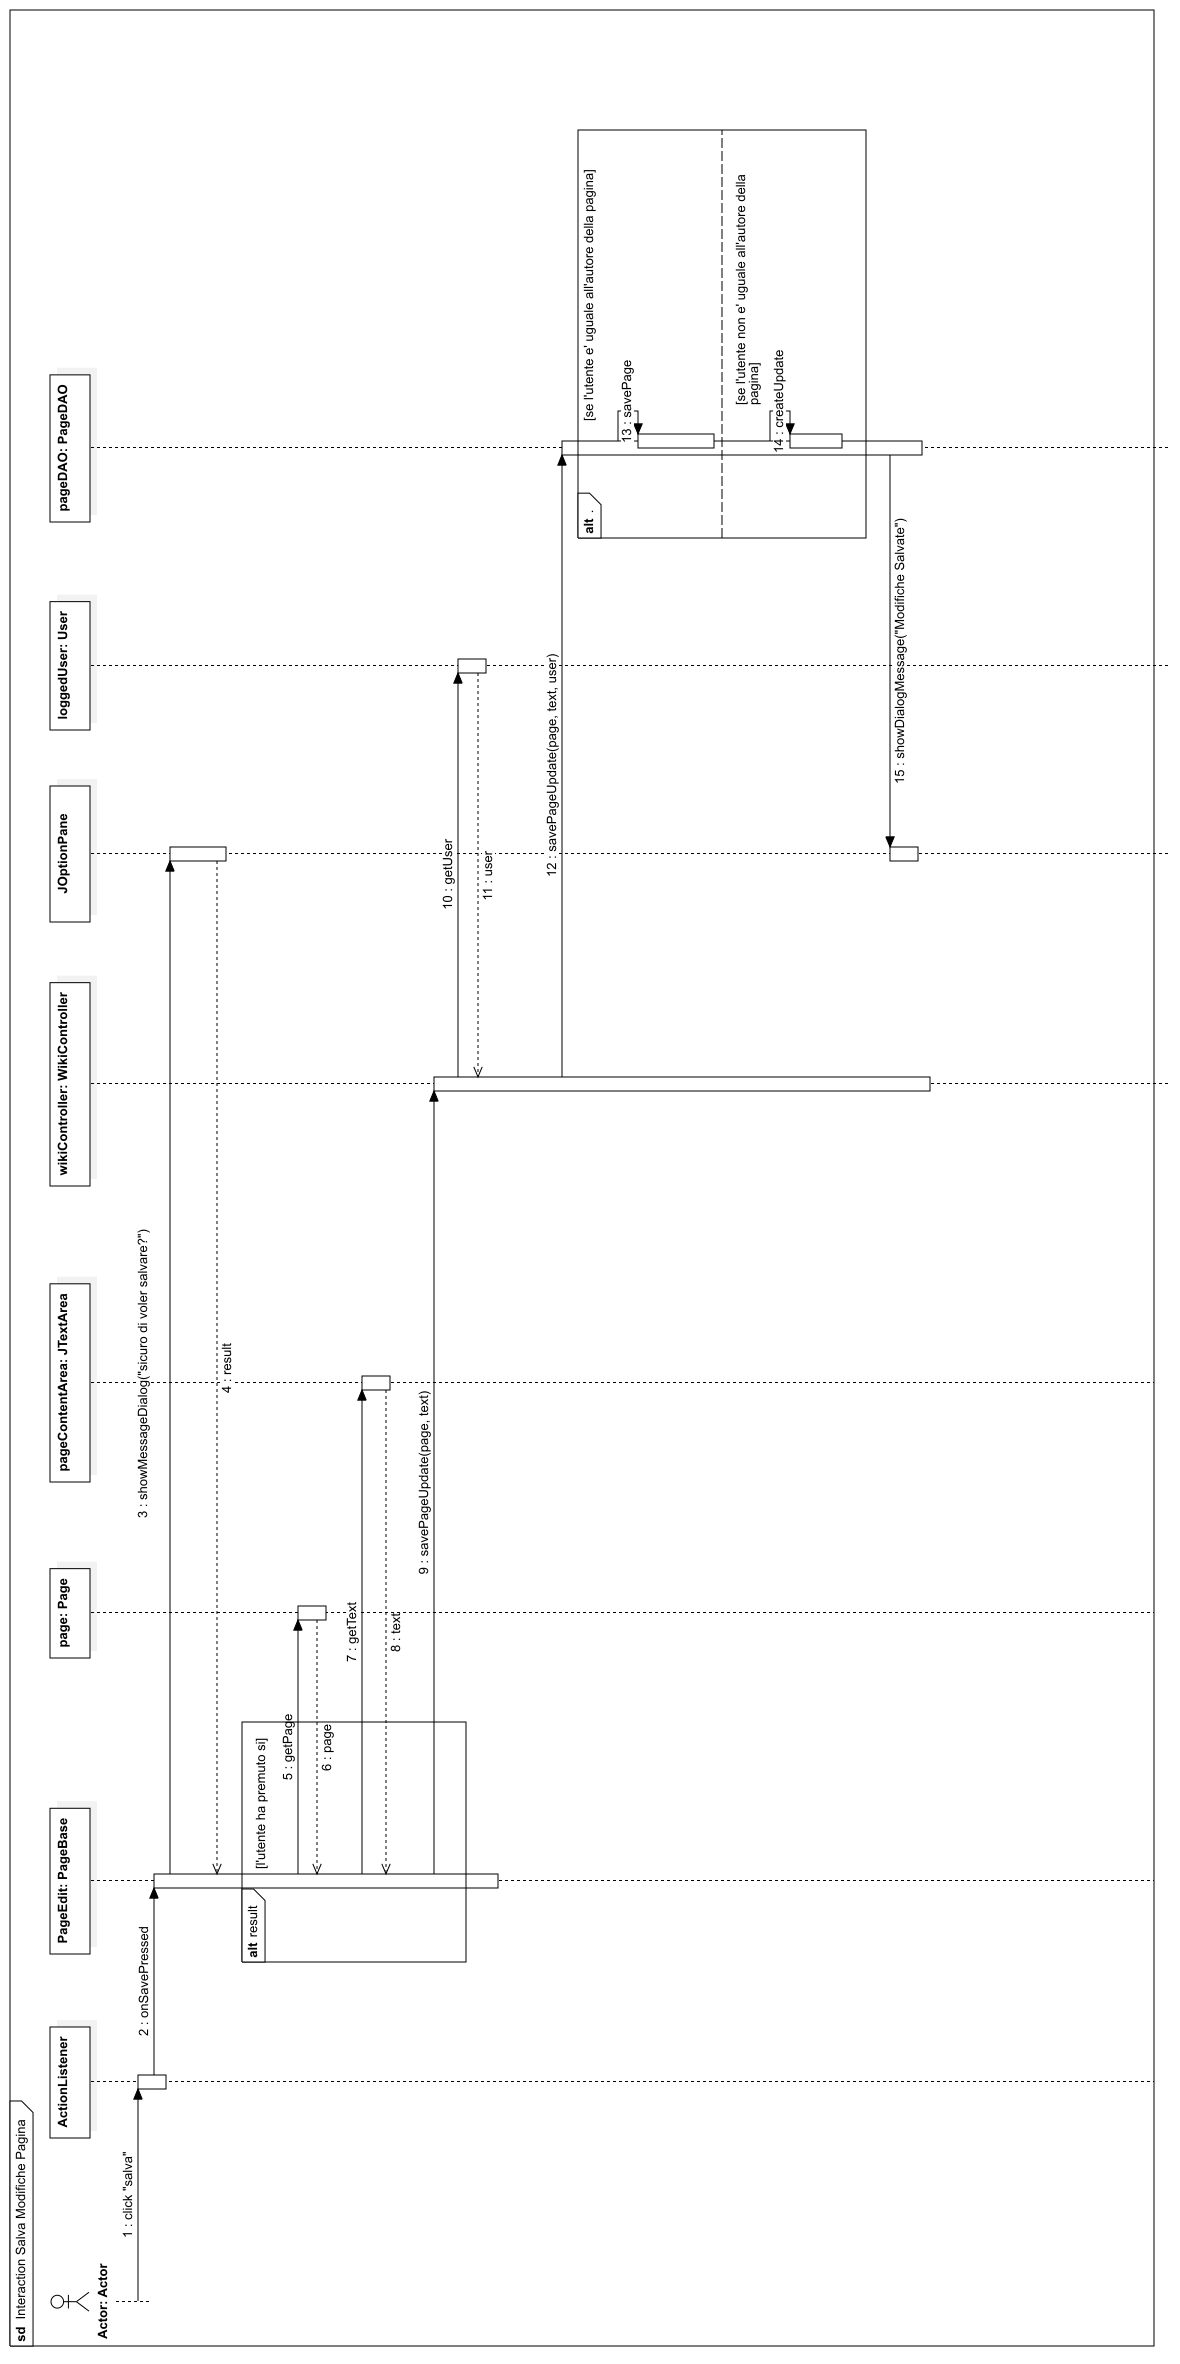
\includegraphics[width=0.7\textwidth,height=0.7\textheight,keepaspectratio]{sequence_edit.png}
		\label{fig:10}
	\end{figure}
	
\end{document}